\documentclass[12pt]{report}

\usepackage[hidelinks]{hyperref}
\usepackage{graphicx}
\usepackage{cite}
\usepackage[toc,page]{appendix}
\usepackage{longtable}
\usepackage{multirow, array}
\usepackage{float}




\title{Classroom Management Handbook}
\author{Lyron Winderbaum}

\begin{document}

\maketitle

\tableofcontents

\chapter{Introduction}

This document is written as a reference manual of strategies for classroom behaviour management. The goal is that a teacher could consult this document in order to prompt them to think of strategies they could implement in their classroom.

This handbook is organised in chapters. Chapters \ref{chap:preventative}, \ref{chap:supportive} and \ref{chap:corrective} form a list of strategies, each as a section or sub-section therein.
This list is not intended to be comprehensive. These chapters separate strategies into the three broad categories of \cite{Charles2002}: preventive, supportive, and corrective, respectively. The description of each strategy is as minimal as possible. Further discussion of examples and theory are left for later chapters and appendices. Some strategies fall in multiple categories. I will include an entry for a strategy in multiple chapters only if I deem that their use (or purpose) is so different in the different categories context that they warrant consideration as separate strategies. Chapter \ref{chap:video_examples} aligns some of the videos shown in lectures to these strategies, and Appendix \ref{app:videos} includes synopses and more detailed discussion of these videos. Chapter \ref{chap:theories} introduces a selection of theorists, their theories, and how they relate to the listed strategies.

\textbf{Disclaimer 1:} I've written this document from my perspective, so any statements that are not explicitly referenced to be otherwise are my personal opinion and nothing more.

\textbf{Disclaimer 2:} In some places I might use language such as ``It is wrong to...'', ``You should...'', etc. --- it is important to recognise that every situation comes with it's own intricacies and context and that no such absolute statements can ever be universal.

Word Count: 3080\footnotemark 

\footnotetext{I shit you not. The words "Word Count: 3080" literally brought it up from 3077 to 3080. This word count is not including title page, table of contents, page numbers, footnotes, captions, refernces, section and chapter numbers (i.e. ``Chapter 1: Introduction'' would count for one word, ``Chapter 2: Preventive Strategies'' would count for two words), and it also doesn't count inline references, either to external sources or in-text hyperlinks (so all the section number refernces are not included. If you don't believe me (I barely believe me) you can access a text-only version \href{https://github.com/Armadilloa16/eportfolio/blob/gh-pages/files/assignments/handbook/files/Handbook_textonly.docx}{at this link}.}






\chapter{Preventative Strategies}
\label{chap:preventative}

Are preventative in the sense that they describe strategies that can help prevent misbehaviour occurring in the first place. These are by far the most preferable strategies to be using and so should always be the place to start.

\section{Praise}
\label{sec:praise_p}

Praise your students! Some students may never have been praised before, don't underestimate the power it can have. \textbf{Be specific} --- praise some work they have done, or how they self regulated. But most importantly: \textbf{be genuine}, if you are not, your students will know.



\section{Show Interest}
\label{sec:show_interest_p}

Be interested in what is going on in your students lives. This is a natural extension of not assuming and being compassionate (\ref{sec:compassion_s}), but can also lead to learning about what is important to your students and this can allow you to design relevant (\ref{sec:relevance_p}) and interesting (\ref{sec:fun_p}) lessons for them.



\section{Use Names}
\label{sec:use_names_p}

Learn the students names. Use them. Students will appreciate the effort you demonstrated by putting in the work (\ref{sec:show_interest_p}). Similarly to praise (\ref{sec:praise_p}), the impact of this strategy is not to be underestimated.

\textbf{Supportive:} Using names can also be used to reinforce supportive strategies such as praising peers (\ref{sec:acknowledge_good_behaviour_s}) by showing that you are not only noticing a students on-task behaviour, but remembering that specific students name.



\section{Rapport with Students}
\label{sec:rapport_p}

Praise (\ref{sec:praise_p}), using names (\ref{sec:use_names_p}) are both ways of showing interest (\ref{sec:show_interest_p}) in your students. When you do these things you can develop a rapport with the students and that can be a powerful and valuable thing.



\section{Establish Routines and Procedures}
\label{sec:routines_p}

Habit is powerful. If you can instill routines into you class early, you can save yourself alot of headache in the future.

\subsection{Democratic Setting of Classroom Practices}
\label{sec:democratic_setting_of_routines_p}

Discuss classroom practices with students --- give them an opportunity to share their opinions. If they buy into the rules and routines by having influence on deciding what they are, they will have a sense of ownership, and be more likely to follow those rules and routines.

\subsection{Set Clear Expectations}
\label{sec:set_clear_expectations_p}

Once the `rules' of the class have been established, either by you or by democratic process with the class (\ref{sec:democratic_setting_of_routines_p}), ensure to communicate them clearly (\ref{sec:clear_instructions_p}) and enforce them consistently.



\section{Use of Language}
\label{sec:language_p}

The words we choose and the way we speak can have a profound impact on how people perceive us, and students can be particularly sensitive to this.

\begin{itemize}
  \item Use inclusive language --- don't assume (\ref{sec:compassion_s})!
  \item Use clear and concise sentences.
  \item Use appropriate vocabulary.
  \item Articulate well, and at an appropriate volume.
  \item If you have any English as an additional language students, or students with hearing impairments, ensure they have access to the information: 
  \begin{itemize}
    \item Use sign language (if possible), 
    \item Provide translations (if possible), 
    \item Speak slowly and clearly, 
    \item Articulate deliberately,
    \item Do the above without being condescending.
  \end{itemize}
\end{itemize}

\subsection{Clear Instructions}
\label{sec:clear_instructions_p}

It is particularly crucial to be clear when delivering instructions. For verbal instructions,
\begin{itemize}
  \item Be heard: Ensure there is silence before delivering instructions (same as \ref{sec:start_well_p}).
  \item Ensure students have access to all the information they need: If you are asking them to interpret an image, ensure they can see the image, etc. 
  \item Use clear verbs so it is clear what is expected of them (\ref{sec:set_clear_expectations_p}): ``Calculate'', ``Write'', etc.
\end{itemize}

\subsection{Clear Materials}
\label{sec:clear_materials_p}

Delivering instructions clearly equally applies to written instructions, not only verbal instructions (\ref{sec:clear_instructions_p}, \ref{sec:set_clear_expectations_p}). This means using appropriate fonts and vocabulary, etc.



\section{Non-verbals}
\label{sec:non_verbals_p}

Similar to the use of language (\ref{sec:language_p}), non-verbals such as body language, positioning, attitude, facial expressions, etc. have a big impact on how you are perceived. 

\subsection{Enthusiasm}
\label{sec:enthusiasm_p}

The students can tell if you are genuinely enthusiastic about the lesson, about the topic, about seeing them, and enthusiasm is infectious.



\section{Preparation}
\label{sec:preparation_p}

This is an important strategy. If you put in work preparing for your classes, it will pay off both because of the preparation itself, but also because your students will recognise the work you have put in for them, and appreciate it. 

\subsection{Relevance}
\label{sec:relevance_p}

Design material (lessons, activities, etc.) that is relevant to your students lives. If you have some rapport (\ref{sec:rapport_p}) with your students you can ask them what they are interested in and design lessons and activities around their interests.

\subsection{Fun}
\label{sec:fun_p}

Design interesting and fun lessons and activities! Similar to relevance (\ref{sec:relevance_p}) if you have some rapport (\ref{sec:rapport_p}) with your students you could try asking them what they think might be fun and try designing a lesson around that.

\subsection{Variety}
\label{sec:variety_p}

If you do the same kind of activity over and over, it will get boring. Mix it up! Use a variety of approaches and activities both within a class and across classes (\ref{sec:kounin_theory}, \ref{sec:blooms_taxonomy}, \ref{sec:gardner_theory}).

\subsection{Structure}
\label{sec:structure_p}

Design structured lessons. This is vague and broad, but having prepared an appropriate amount of activities and a structure linking them together in a lesson cannot be overstated \ref{sec:kounin_theory}.



\section{Lesson Movement / Momentum}
\label{sec:flow_p}

Having multiple different activities in your lessons is important (\ref{sec:variety_p}, \ref{sec:kounin_theory}). Be aware of transitions between activities. Insist on silence and attention before you deliver instructions for the next activity (\ref{sec:clear_instructions_p}), and work this into a class routine (\ref{sec:routines_p}).

\subsection{Start Well}
\label{sec:start_well_p}

Starting the class represents a big transition: from out-of-class to in-class, and so you should ensure to managed it the same way (\ref{sec:flow_p}). This is a particularly important routine (\ref{sec:routines_p}) to set. One way to manage the start of a lesson in a structured way (\ref{sec:structure_p}) is to use a starter activity. A starter is a short (5-10min) activity that is fun, engaging, and easy, and serves the function of settling the class.




\section{Time Management}
\label{sec:manage_your_time_p}

Reflect on how you have been spending your time in class, and if necessary make adjustments. 



\section{Model Appropriate Behaviors}
\label{sec:model_behaviours_p}

Don't be a hypocrite. If you ask the students to behave a certain way --- adhere to the same standard yourself.


























\chapter{Supportive Strategies}
\label{chap:supportive}

Are for situations when misbehavior is occuring but is not so severe as to require being addressed directly. Supportive strategies aim to encourage and guide students towards adopting more productive and helpful behaviours. 


\section{Praise}
\label{sec:praise_s}

Although praise can be preventative (\ref{sec:praise_p}), it can also be used as a supportive strategy. For students who sometimes meander off task, praising their on-task behaviour can encourage more on-task behaviours.

\subsection{Peer Praise}
\label{sec:peer_praise_s}

One of the strongest forms of praise you can offer a student is that of their peers --- if a student has done something particularly well, encourage their peers to applaud, or similar.
Warning: certain types of students may react badly to this, use with discretion.

\subsection{Praise Peers}
\label{sec:acknowledge_good_behaviour_s}

Misbehaviour motivated by wanting your attention can be managed by praising other on-task students combined with carefully not giving attention to the misbehaviour (\ref{sec:tactical_ignoring_s}).



\section{Be Compassionate}
\label{sec:compassion_s}

You don't know what your students have gone through at home or in their lives. You don't know if their misbehaviour is malicious or is just coming from learnt emotional reactions they have no control over. \textbf{Don't assume}. Train your initial reflex reaction to misbehaviour to be one of compassionate calm. This has the potential to open a door to building rapport (\ref{sec:rapport_p}). It can also help in giving \textbf{genuine} praise (\ref{sec:praise_p}) and showing interest (\ref{sec:show_interest_p}).

This strategy is obviously easier said than done, but it is an important one to keep in the back of your mind as you work on your personal development.



\section{Scaffolding}
\label{sec:scaffolding_s}

If students are losing interest and going off-task as a result of trying, but struggling to complete, a task --- offer to help (scaffold) them in completing the task (\ref{sec:zpd_theory}). If you can give them a sense of success and accomplishment by helping them complete the task, this can encourage future on-task behaviour.



\section{Proximity (``The Whisper Technique'')}
\label{sec:proximity_s}

Proximity can be used as a supportive strategy by using it to deliver help (\ref{sec:scaffolding_s}) privately. Often if you offer help publically (in front of the students classmates) it can be embarrassing for them and they might not be receptive. In contrast, using proximity to deliver aid in a whisper that is not as public can improve the chances that the student will be receptive to the scaffolding.

\textbf{Corrective:} Proximity can also be used to deliver correctives, either a soft corrective simply by placing yourself (the teacher) near the misbehaviour to deter it\footnotemark, or by whispering an admonishment or a direct appeal (\ref{sec:direct_appeal_c}). Warning: Proximity can be very intimidating and can prompt a strong response in students if used in the wrong circumstances or with the wrong student --- use discretion.

\footnotetext{As with most soft correctives the best use would be seamlessly interwoven into your delivery without impacting on the flow of the lesson (\ref{sec:flow_p}, \ref{sec:kounin_theory}).}

\section{Distraction}
\label{sec:distraction_s}

Distract the misbehaving student by giving them something unrelated and interesting to engage their attention.



\section{Tactical Ignoring}
\label{sec:tactical_ignoring_s}

This is the other half of the coin to praising peers (\ref{sec:acknowledge_good_behaviour_s}) when dealing with attention seeking students. You can deliberately ignore off-task behaviour, giving your attention instead to on-task behaviour and the misbehaving students may begin to feel left out, and start to cooperate in an attempt to be included.



\section{Wait Time}
\label{sec:wait_time_s}

Broken sentences --- pause to get attention if students are misbehaving to signal them to stop. This is one of those borderline correctives, also called ``Canter's ``Broken Record'''' in Figure~\ref{fig:correctiveHierarchy}.


\section{Challenge Students}
\label{sec:challenge_s}

Particularly if you suspect the misbehaviour is motivated from boredom, issue a challenge to the misbehaviours to complete some task --- preferably a relevant and engaging task (\ref{sec:relevance_p}, \ref{sec:fun_p}) that will challenge them. 



\section{Use Humour to Depotentiate}
\label{sec:humour_s}

Is a students misbehaviour has led to confrontation or tension in the classroom, try using humour to depotentiate the situation.

























\chapter{Corrective Strategies}
\label{chap:corrective}

Are for the times when students misbehave to a point that their misbehaviour must be addressed directly and can no longer be managed by supportive strategies alone. The central thinking when implementing a corrective should always be to avoid escalation. The harsher the corrective used, the more likely it is to result in escalation, and so it is always preferable to use the softest corrective possible that manages the behaviour. See Figure~\ref{fig:correctiveHierarchy}.

It is also important to note the special case of chronic misbehaviour --- in this case it is particularly important to try to understand the underlying cause of the misbehaviour, for which Dreikurs' social discipline model (\ref{sec:dreikur_theory}) can be particularly helpful. Hence I have incorporated my discussion of strategies for managing chronic misbehaviour into section \ref{sec:dreikur_theory}.


\begin{figure}[p]
\begin{center}
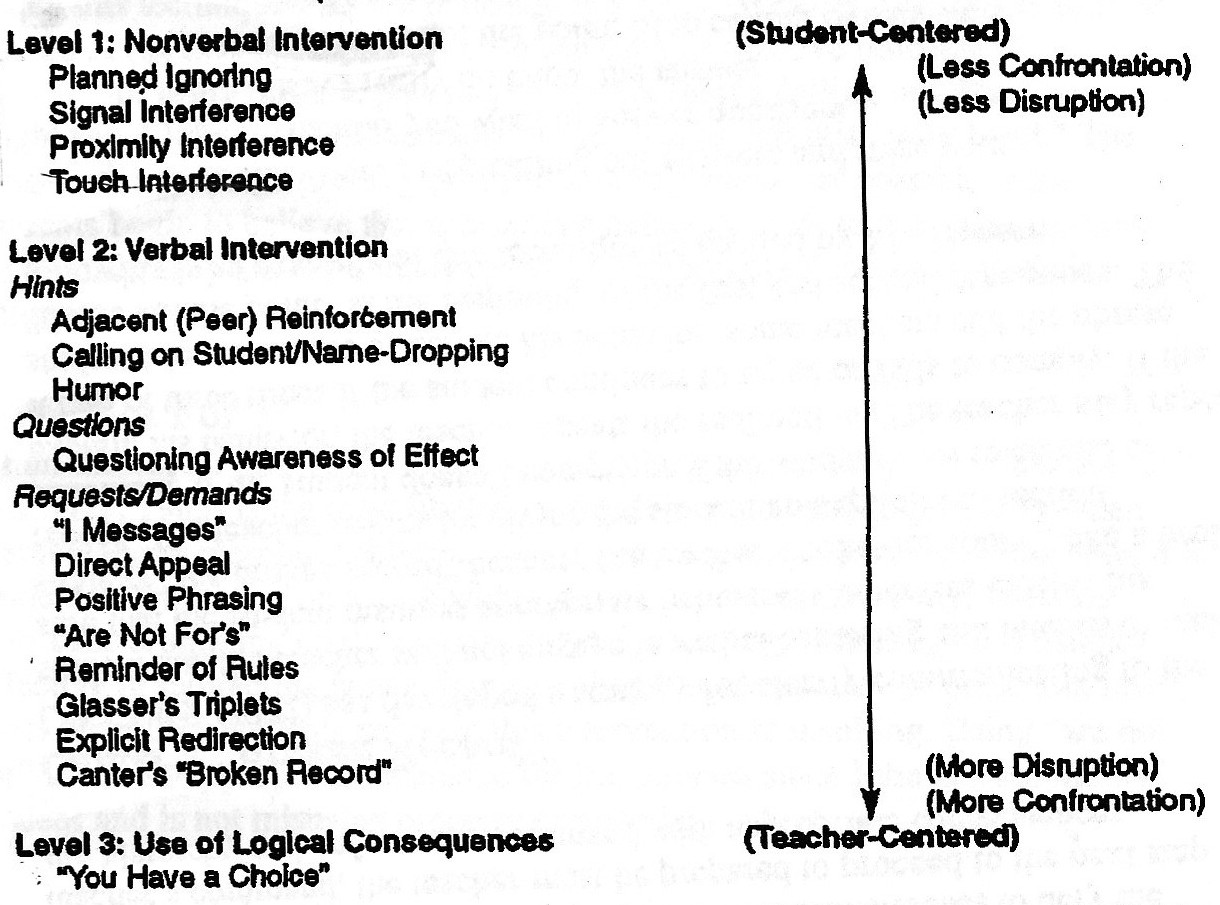
\includegraphics{./images/correctiveHierarchy.jpg}
\end{center}
\caption{Hierarchy of Management Intervention Diagram \cite{Levin2005} showing a list of corrective strategies, ranked in increasing order of harshness. Some of these are not applicable (such as touch), and others have already been covered as supportive strategies such as "Planned Ignoring" (\ref{sec:tactical_ignoring_s}), "Proxomity Interference" (\ref{sec:proximity_s}), "(Peer) Reinforcement" (\ref{sec:peer_praise_s}), and "Humour" (\ref{sec:humour_s}), as there is a grey area between supportive and soft corrective strategies. \label{fig:correctiveHierarchy}}
\end{figure}


\section{Eye Contact}
\label{sec:eye_contact_c}

Catch the misbehaving students' eye from across the room and hold their gaze for a moment\footnotemark. 



\section{Calling on Student}
\label{sec:use_names_c}

Call out the misbehaving student by name\footnotemark[\value{footnote}].



\footnotetext{As with most soft correctives the best use would be seamlessly interwoven into your delivery without impacting on the flow of the lesson (\ref{sec:flow_p}, \ref{sec:kounin_theory}).}



\section{Questioning Awareness of Effect}
\label{sec:questioning_c}

Ask the misbehaving student if they are aware of the effect their behaviour is having on the class or surrounding students\footnotemark.



\section{Gordons I-Messages}
\label{sec:i_messages_c}

Gordon (\ref{sec:gordon_theory}) suggested a three step process for initiating a conversation with a student in a non-confrontational\footnotemark[\value{footnote}] way (at least that is the intention!)  about behaviour the teacher is unhappy with:
\begin{itemize}
  \item Describe the disruptive behaviour.
  \item Describe the effect on the teacher and/ or other students.
  \item Describe your feelings about the behaviour.
\end{itemize}



\section{Reminder of Rules}
\label{sec:reminder_c}

Remind the student, by name (\ref{sec:use_names_c}), of the rule they are in violation of. Note that these rules should have already been clearly (\ref{sec:language_p}) set out previously (\ref{sec:routines_p}) --- that they are breaking\footnotemark[\value{footnote}].



\section{Direct Appeal}
\label{sec:direct_appeal_c}

Tell the student, by name (\ref{sec:use_names_c}), to stop the misbehaviour. Note: do not ask or use "please", you are giving a directive\footnotemark[\value{footnote}].



\section{Glassers Triplets}
\label{sec:glassers_triplets_c}

Are three questions that can be posed to a student to answer:
\begin{itemize}
  \item What are you doing?
  \item Is that against the rules?
  \item What should you be doing instead?
\end{itemize}
If the student is being uncooperative, instead of engaging in a confrontation 
you should simply state the answers to these questions and move on\footnotemark[\value{footnote}].



\section{Private Talk}
\label{sec:private_talk_c}

Arrange for a time out of class to talk with the student or students. Often it might be easiest to ask them to stay after class\footnotemark[\value{footnote}]. This would be one of my preferred correctives, should a strong corrective be needed. 

\footnotetext{Having some rapport (\ref{sec:rapport_p}) with the student can greatly increse the chances of a successful outcome from stronger corrective strategies such as these.}


\section{Give Choice}
\label{sec:give_choice_c}

Give the misbehaving student a choice: either stop the misbehaviour, or suffer a consequence. 

\section{Apply Sanctions}
\label{sec:sanctions_c}

If the student has:
\begin{itemize}
  \item been given a choice (\ref{sec:give_choice_c}) and chosen not to stop the misbehaviour, or 
  \item broken an established rule (\ref{sec:routines_p}) either defined by you, the school, or by the class (\ref{sec:democratic_setting_of_routines_p}), 
\end{itemize}
then you must deliver the consequence, which could be anywhere from staying back after class, having a chat with you (\ref{sec:private_talk_c}), being ejected from the class, detention, or even exclusion or suspension.














\chapter{Video Examples}
\label{chap:video_examples}

In the interests of brevity, all I will present here is a table showing the correspondence between the video examples and the strategies. This is intended to allow a teacher interested in a particular strategy to quickly and easily identify which videos are relevant to that strategy. I have written more detailed synopses and reviews of these videos, including specific time-stamps for various key points discussed, see Appendix~\ref{app:videos}. Infact, I use the section numbering of Appendix~\ref{app:videos} to identify the videos in Table~\ref{tab:videos}

\pagebreak
\begin{longtable}{rl|c|c|c|c|c|c|c|}

 & & \multicolumn{7}{|c|}{Video} \\
 & Strategy & \ref{video:1} & \ref{video:2} & \ref{video:3} & \ref{video:4} & \ref{video:5} & \ref{video:6} & \ref{video:7} \\ \hline
\endhead
\parbox[t]{2mm}{\multirow{21}{*}{\rotatebox[origin=c]{90}{Preventive Strategies}}}
& \ref{sec:praise_p}  Praise                                   &X& & &X&X& & \\
& \ref{sec:show_interest_p} Show Interest                             & & & &X& & & \\
& \ref{sec:use_names_p} Use Names                                 & & & & & & &X\\
& \ref{sec:rapport_p} Rapport with Students                                   & & & &X& &X&X\\
& \ref{sec:routines_p}  Establish Routines ...                              &X& & & & & &X\\
& \hspace{6pt}\ref{sec:democratic_setting_of_routines_p} Democratic ... & &X& & & & & \\
& \hspace{6pt}\ref{sec:set_clear_expectations_p} Set Clear Expect...       & & & & & & &X\\
& \ref{sec:language_p} Use of Language                                   & &X& & & & &X\\
& \hspace{6pt}\ref{sec:clear_instructions_p} Clear Instructions             & &X& & & & &X\\
& \hspace{6pt}\ref{sec:clear_materials_p} Clear Materials                &X& & & & & & \\
& \ref{sec:non_verbals_p} Non-verbals                                &X&X&X&X& & &X\\
& \hspace{6pt}\ref{sec:enthusiasm_p} Enthusiasm                    & & & & & & & \\
& \ref{sec:preparation_p} Preparation                                 &X& & &X&X& &X\\
& \hspace{6pt}\ref{sec:relevance_p} Relevance                      & & & &X&X& & \\
& \hspace{6pt}\ref{sec:fun_p} Fun                            & & & & &X& &X\\
& \hspace{6pt}\ref{sec:variety_p} Variety                        & & & &X& & & \\
& \hspace{6pt}\ref{sec:structure_p} Structure                      &X& & & & & & \\
& \ref{sec:flow_p} Lesson Movement ...                                       &X& & & & & & \\
& \hspace{6pt}\ref{sec:start_well_p} Start Well                     & & & & & & & \\
& \ref{sec:manage_your_time_p} Time Management                           & & & & & &X& \\
& \ref{sec:model_behaviours_p} Model Appropriate ...                          & & & & & & & \\
\hline
 & & & & & & & & \\
 & & & & & & & & \\ \hline
\parbox[t]{2mm}{\multirow{11}{*}{\rotatebox[origin=c]{90}{Supportive Strategies}}}
& \ref{sec:praise_s} Praise                                     &X&X&X&X&X& & \\
& \hspace{6pt}\ref{sec:peer_praise_s} Peer Praise                    &X&X& &X& & & \\
& \hspace{6pt}\ref{sec:acknowledge_good_behaviour_s} Praise Peers     & & & & &X& & \\
& \ref{sec:compassion_s} Be Compassionate                                 & & & & & & & \\
& \ref{sec:scaffolding_s} Scaffolding                                & &X& & & & & \\
& \ref{sec:proximity_s} Proximity ...                                  &X&X&X& &X& &X\\
& \ref{sec:distraction_s} Distraction                                & & & & & & & \\
& \ref{sec:tactical_ignoring_s} Tactical Ignoring                          & & & & &X& & \\
& \ref{sec:wait_time_s} Wait Time                                  & & &X& & & &X\\
& \ref{sec:challenge_s} Challenge Students                                  & & & & & & & \\
& \ref{sec:humour_s} Use Humour ...                                  & & & & & & &X\\
\hline
 & & & & & & & & \\ 
 & & & & & & & & \\ 
\parbox[t]{2mm}{\multirow{10}{*}{\rotatebox[origin=c]{90}{Corrective Strategies}}}
& \ref{sec:eye_contact_c} Eye Contact                                & & & & & & &X\\
& \ref{sec:use_names_c} Calling on Student                                  & & &X& &X& & \\
& \ref{sec:questioning_c} Questioning ...                                & & & & & & & \\
& \ref{sec:i_messages_c} Gordons I-Messages                                 & & & & & & & \\
& \ref{sec:reminder_c} Reminder of Rules                                   & & & & & & & \\
& \ref{sec:direct_appeal_c} Direct Appeal                              & & &X& &X& & \\
& \ref{sec:glassers_triplets_c} Glassers Triplets                          & & & & & & & \\
& \ref{sec:private_talk_c} Private Talk                               & & &X& & & & \\
& \ref{sec:give_choice_c} Give Choice                                & & &X& & & & \\
& \ref{sec:sanctions_c} Apply Sanctions                                  & & &X& & & & \\
\hline 
\caption{Note there is an inherent bias in the data presented here for strategies I am more familiar with and comfortable with, as I recognised them more easily in the videos. Even now, writing this, I am still thinking of strategies in these videos that I missed. So there is no way I could realistically claim this is in any way comprehensive. Each example of a strategy marked in this table is certainly there, but there are (I guarantee) strategies in the videos not marked in this table. Instead, consider this table as a guide for highlighting key differences of focus between the videos covered: notice, for example, how \ref{video:3} and \ref{video:5} explore corrective strategies more than the others. Notice how comprehensively \ref{video:7} covers preventative strategies, etc.
\label{tab:videos}}

\end{longtable}










































\chapter{Theories and Theorists}
\label{chap:theories}

In this chapter I discuss a selection of theories and theorists.

% For more see Appendix~\ref{app:theory}.



\section{Skinners' Operant Conditioning}
\label{sec:skinner_theory}

Burrhus Frederic Skinner is attributed to the version of behaviorism ``radical behaviorism'' \cite{Skinner2011} and amongst other things developed ``operant conditioning'' \cite{Skinner1950} beyond the initial work of Edward Lee Thorndike \cite{Thorndike1898}. In the context of teaching operant conditioning is typically implemented through extrinsic motivators. That is, the ``carrot and stick'' concept. In practice this will involve reinforcement either positive (rewards such as praise (\ref{sec:praise_s}) are given for the desired behaviour), or negative (retract sanctions (\ref{sec:sanctions_c}) as a reward for the desired behaviour).



\section{Thomas Gordon}
\label{sec:gordon_theory}

The approach of Thomas Gordon came to be known as "the Gordon Model", and is centred on "the importance of developing meaningful mutually beneficial relationships" [\href{https://en.wikibooks.org/wiki/Classroom_Management_Theorists_and_Theories/Thomas_Gordon}{wiki page}]. Gordon believed that in relationships each party (in our case students and teachers) bring their own values and needs, and that these will inevitably not match and result in conflict. Gordon suggested that to resolve such conflicts the first step is to identify who "owns" the problem --- that is in essence, which is the disgruntled party. Then:
\begin{itemize}
  \item If the student "owns" the problem, the teacher should engage in "active listening" --- that is they should listen to the students grievance and genuinely try to understand and empathise with their frustrations (\ref{sec:show_interest_p}, \ref{sec:compassion_s}, \ref{sec:non_verbals_p}).
  \item If the teacher "owns" the problem, then they should use an "I-message" (\ref{sec:i_messages_c}) to initiate a conversation in a non-confrontational way.
\end{itemize}
Finally, the objective in Gordons framework is to achieve a solution in which both parties have contributed and feel invested in, similar in principle to the buy-in discussed in \ref{sec:democratic_setting_of_routines_p}.



\section{Vygotsky's ZPD}
\label{sec:zpd_theory}

The Zone of Proximal Development or ZPD was first proposed by Lev Vygotsky, who defined it as

\begin{quote}
`` ... the distance between the actual development level as determined by independent problem solving and the level of potential development as determined through problem solving under adult guidance or in collaboration with more capable peers.''

\hfill \cite{Vygotsky1978}
\end{quote}

Although the concept has been developed further since, the basic principle remains very close to the original proposed by Vygotsky, and fits well with the broader philosophy of constructivism. 

The key consequence for teachers is that according to this constructivist model, all learning occurs in the ZPD. In essence, this puts the concept of scaffolding (\ref{sec:scaffolding_s}) front and centre to all teaching and learning efforts. In order to maintain engagement and deliver effective teaching, students need to be kept in the ZPD by careful planning of lessons (\ref{sec:preparation_p}) and provision of appropriate scaffolding (\ref{sec:scaffolding_s}).



\section{Jacob Kounin}
\label{sec:kounin_theory}

Jacob Kounin suggested good ``Lesson Movement'' is needed for effective teaching. This means, amongst other things, regular transitions between activities: the same activity over long periods would get stale (\ref{sec:variety_p}, \ref{sec:flow_p}). Kounin suggested that in order to achieve good lesson movement, five components where needed: ``withitness'' (a term he coined), overlapping, momentum, smoothness, and group focus. Each of these has its own subtleties in Kounin's theories, but in essence, they sum to an awareness of the class and an ability to intercede and prevent misbehaviours before they occur. Kounin also wrote alot about the effect a teacher can have on misbehaviour in their class through mostly preparatory techniques (\ref{sec:preparation_p}) such as structuring lessons well (\ref{sec:structure_p}).

\section{Dreikurs' Social Discipline Model (in the context of chronic misbehaviour management)}
\label{sec:dreikur_theory}

Dreikurs' ``Social Discipline Model'' claims that the goal of misbehavior is usually one of:
\begin{itemize}
  \item attracting attention,
  \item power,
  \item revenge, or
  \item escape by withdrawal.
\end{itemize}
and that which one it is likely to be can be diagnosed by observing the effect the behaviour has on the teacher. If the teacher feels:
\begin{itemize}
  \item Minor annoyance and frustration, the goal is attention seeking.
  \item Personally challenged, the goal is power. 
  \item Deeply hurt, the goal is revenge.
  \item Like giving up, the goal is escape by withdrawal.
\end{itemize}
The two most common goals are attracting attention, and escape by withdrawal. There are two broad approaches to addressing chronic misbehaviour, which can roughly be matched against these two goals respectively:
\begin{itemize}
  \item Relationship Building: through building rapport (\ref{sec:rapport_p}) and having private conversations (\ref{sec:private_talk_c}) with the student, often acceptable behaviours can be negotiated where both the teachers and the students needs are being met.
  \item Breaking the cycle of discouragement: through scaffolding (\ref{sec:scaffolding_s}), careful design of lessons and praise (\ref{sec:praise_s}), the student can be given a feeling of success which can sometimes break through their cycle of discouragement.
\end{itemize}
  








\begin{appendices}

\chapter{Video Example Synopses}
\label{app:videos}

This appendix contains my synopses and reviews of the video examples of teaching practice, organised into sections. There is one additional section, Section~\ref{video:other}, which contains a list of videos I have not yet reviewed.

\section{Praise and Preparation}
\label{video:1}

\href{https://www.youtube.com/watch?v=KkXRjrSsMQg}{This ``Teaching with Bayley'' clip} shows Queensland teacher Amy Alexander teaching seventh grade at Pimlico School. Amy explains how ``These kids respond well to praise. I think at home they're being told how terrible they are'' (\href{https://www.youtube.com/watch?v=KkXRjrSsMQg&t=235}{3:55}). Amy uses non-verbals (\ref{sec:non_verbals_p}) such as being happy to see the class straight off the bat (\href{https://www.youtube.com/watch?v=KkXRjrSsMQg&t=55}{0:55}). She also comes right off the bat using names (\href{https://www.youtube.com/watch?v=KkXRjrSsMQg&t=101}{1:41}, \href{https://www.youtube.com/watch?v=KkXRjrSsMQg&t=120}{2:00}) and continues using names throughout the class (\href{https://www.youtube.com/watch?v=KkXRjrSsMQg&t=402}{6:42}, \href{https://www.youtube.com/watch?v=KkXRjrSsMQg&t=731}{12:11}, \href{https://www.youtube.com/watch?v=KkXRjrSsMQg&t=749}{12:29}, \href{https://www.youtube.com/watch?v=KkXRjrSsMQg&t=757}{12:37}) mostly to deliver praise, but also instructions, and supportive strategies. Amy delivers her praise in a number of different ways too, as Bayley notes (\href{https://www.youtube.com/watch?v=KkXRjrSsMQg&t=455}{7:35}), she offers class-wide praise for listening and good behaviour (\href{https://www.youtube.com/watch?v=KkXRjrSsMQg&t=433}{7:13}), but also targeted praise to specific students for their behaviour or answers which is sometimes delivered publically (\href{https://www.youtube.com/watch?v=KkXRjrSsMQg&t=100}{1:40}, \href{https://www.youtube.com/watch?v=KkXRjrSsMQg&t=121}{2:01}, \href{https://www.youtube.com/watch?v=KkXRjrSsMQg&t=125}{2:05}, \href{https://www.youtube.com/watch?v=KkXRjrSsMQg&t=401}{6:41}), even encouraging peer praise (\ref{sec:peer_praise_s}) for a particularly good answer (``give that answer a round of applause please'', \href{https://www.youtube.com/watch?v=KkXRjrSsMQg&t=200}{3:20}), and also using proximity (\ref{sec:proximity_s}) to deliver praise (\ref{sec:praise_s}) as a supportive (\href{https://www.youtube.com/watch?v=KkXRjrSsMQg&t=615}{10:15}). Amy also talks about how she has ``gotta keep them moving'', reinforcing the importance of flow (\ref{sec:flow_p}), and makes this much easier on herself by writing instructions on the board before the class has even started (\ref{sec:preparation_p}, \href{https://www.youtube.com/watch?v=KkXRjrSsMQg&t=38}{0:38}) freeing her up during class to focus on managing behaviour, and using a consistent colour-coding system every class so the students quickly become familiar with the system and know what to expect (\ref{sec:routines_p}, \ref{sec:structure_p}, \ref{sec:clear_materials_p}). Overall Amy demonstrates what is inarguably a master-class in the use of preparation (\ref{sec:preparation_p}), structure (\ref{sec:structure_p}) and most of all praise (\ref{sec:praise_p}) to manage what would otherwise be a very difficult class. 



\section{Too Much Talk}
\label{video:2}

\href{http://archive.teachfind.com/ttv/www.teachers.tv/videos/too-much-talk.html}{This ``Teaching with Bayley'' clip} shows geography John Fuentes teaching at Bexleyheath School. Initially Johan is shown struggling with some basic strategies: 
\begin{itemize}
  \item He moves around alot and Bayley suggests adopting a `teaching position'' (2:40, \ref{sec:non_verbals_p}).
  \item He repeatadly says ``Ok?'', communicating a lack of confience and undermining his own delivery (3:20, \ref{sec:language_p}).
  \item He fails to transition when the class begins to lose interest, and then when he does he doesn't have their attention and so his instructions are unclear (4:50, \ref{sec:clear_instructions_p}).
\end{itemize}
On a positive note however, he negotiates with the students on how much time to give them to complete a task (7:00, \ref{sec:democratic_setting_of_routines_p}). After some reflection, John decides he is going to focus on talking less himself, and involving specifc students more. He picks out a particular student, Charlie, and asks him to explain a concept (9:26), but when Charlie cannot he offers to let Charlie handball the question to another student Charlie thinks might know the answer (10:08). Later, John comes up to Charlie and offers him some tutoring on the topic (11:26, \ref{sec:proximity_s}, \ref{sec:scaffolding_s}). Then towards the end of the class John goes back to Charlie and asks him another similar question, which (with a little help) Charlie manages to answer (12:30), and gets a round of peer praise for it (\ref{sec:peer_praise_s}). John showed a big improvement between the two classes through involving more student participation and a textbook application of scafolding. Note this strategy of calling out one student can be risky if you don't know th estudents well, certain students might react badly. In this case John seems to know Charlie is a socially confident student, and leverages that.

\textbf{Note:} This link to this video is to \texttt{teachfind.com/ttv/www.teachers.tv/} and not youTube and so I don't know how to make time-stampted hyperlinks, sorry.



\section{Manage that Class}
\label{video:3}

\href{http://archive.teachfind.com/ttv/www.teachers.tv/videos/manage-that-class-year-8-friday.html}{This video} shows a grad teacher Jenny tackling an extremely challenging Friday afternoon year 8 class, with deputy head John Wootton in her earpiece watching over CCTV. She manages the behaviours in the class really well actually, using textbook strategies all the way through, but the class itself is very restless, with a few particular misbehaving students that made it just... a nightmare of a class, to be honest. Right out the door Jenny insists on silence while she is speaking by using a Canter's ``Broken Record'' type approach using names multiple times to interupt her instructions (2:30, 2:40, 2:46, 2:52, \ref{sec:wait_time_s}, \ref{sec:use_names_c}) and when that doesnt seem to be working, she stops instructing entirely and steps aside, using her physical position to indicate she is waiting on the class to quieten (3:10, \ref{sec:non_verbals_p}). John Whootton meanwhile explains that this positioning strategy is a operant conditioning (behaviourism) type approach (3:50, \ref{sec:skinner_theory}), training the students that when she stands in the ``Teaching Position'', they are to give her silence and attention. Througout Jenny is also using praise to point out when students do the right thing (5:25, \ref{sec:praise_s}), and when the problematic student Vulcan plays up also uses proximity as a corrective in an attempt to get him in line (5:40, \ref{sec:proximity_s}), but when that ultimately doesnt work ramps up the harshness of the correctives and gives him a choice (6:02, \ref{sec:give_choice_c}). After transitioning in the lesson, Jenny uses proximity to try and prempt any trouble from the misbehaving students (10:30, \ref{sec:proximity_s}), and towards the end of the class... all hell breaks loose, and she tells the students invovled to stay behind to have a chat with her after class (\ref{sec:private_talk_c}). Phew, what a nightmare of a class. Honestly I think she did great keeping her cool, considering. Friday afternoons with year 8 classes... scary.

\textbf{Note:} This link to this video is to \texttt{teachfind.com/ttv/www.teachers.tv/} and not youTube and so I don't know how to make time-stampted hyperlinks, sorry.





\section{A Lesson From The Best}
\label{video:4}

In \href{https://www.youtube.com/watch?v=zr2xdjQPH4I}{this video} Phillip Beadle showcases two of his classes at Eastlea community school: a year 9 boys class that had been defined as ``potentially at risk of underachieving'' in which they ``Argument Tennis'', and a Year 11 Poery class.

\textbf{``Argument Tennis'':}  The name of the excercise itself relates to competitive sport which probably already appeals to the boys in the class (\ref{sec:relevance_p}), but it also describes how the activity will perform in a funcational sense (hitting the argument back and forth between two players), which would make it very intuitive for the students. Phil uses the competitve aspect to motivate students (\href{https://www.youtube.com/watch?v=zr2xdjQPH4I&t=235}{3:55}), and throughout just provides alot of encouragement both verbally (\href{https://www.youtube.com/watch?v=zr2xdjQPH4I&t=242}{4:02}), but also with his body language (\ref{sec:non_verbals_p}) such as facial expressions (\href{https://www.youtube.com/watch?v=zr2xdjQPH4I&t=309}{5:09}). He also makes use of praise, but in very specific ways to make sure the students know exactly what they are being praise \emph{for} (\href{https://www.youtube.com/watch?v=zr2xdjQPH4I&t=320}{5:20}), with particularly impressive work being rewarded with peer praise (\href{https://www.youtube.com/watch?v=zr2xdjQPH4I&t=383}{6:23}). A real master class.

\textbf{Year 11 Poetry:} He uses visual and audio stimuli (\ref{sec:variety_p}, \href{https://www.youtube.com/watch?v=zr2xdjQPH4I&t=515}{8:35}) to create an intensely engaging context which he then makes relevant using his descriptions (\ref{sec:relevance_p}, \href{https://www.youtube.com/watch?v=zr2xdjQPH4I&t=536}{8:56}). There is almost no misbehaviour, probably at least in part as a consequence of the engaging lesson design, but when there is even very minor misbehaviour Phil delivers correctives so smoothly and without missing a step that you would almost miss it if you blinked (\href{https://www.youtube.com/watch?v=zr2xdjQPH4I&t=609}{10:09}) --- a demonstration is what mastery of ``withitness'' looks like (\ref{sec:kounin_theory}). He also demonstrates a genuine interest in the students, expressing the joy he gets from reading their work (\ref{sec:show_interest_p}, \href{https://www.youtube.com/watch?v=zr2xdjQPH4I&t=822}{13:42}).









\section{Attention Seekers}
\label{video:5}

\href{https://www.youtube.com/watch?v=pXhtwDK4oHw}{This ``Teaching with Bayley'' clip} shows Jane Wright teaching year 7 french at Drayton School in Banbury, Oxfordshire. She is struggling with chronoic low level disruption, still struggling to settle the class 5min in (\href{https://www.youtube.com/watch?v=pXhtwDK4oHw&t=105}{1:45}) after already having used direct appeals (\ref{sec:direct_appeal_c}, \href{https://www.youtube.com/watch?v=pXhtwDK4oHw&t=57}{0:57}) and calling names (\ref{sec:use_names_c}, \href{https://www.youtube.com/watch?v=pXhtwDK4oHw&t=60}{1:00}). When she reflects on her feelings she notes that she feels frustrated (\href{https://www.youtube.com/watch?v=pXhtwDK4oHw&t=120}{2:00}), and in agreement with the theory of Dreikur (\ref{sec:dreikur_theory}) we note there is a group of attention seeking students causing most of the disruption in her class. Bayley suggests using the combined tactical ignoring/ praising peers approach (\ref{sec:tactical_ignoring_s}, \ref{sec:acknowledge_good_behaviour_s}, \href{https://www.youtube.com/watch?v=pXhtwDK4oHw&t=245}{4:05}) as well as suggesting more praise in general (\ref{sec:praise_p}, \href{https://www.youtube.com/watch?v=pXhtwDK4oHw&t=410}{6:50}) and using proximity (\ref{sec:proximity_s}) to deliver correctives so that the delivery of correctives doesn't provide entertainment value to the class because they can't tell if the whisper is directed to the work or the behaviour (\href{https://www.youtube.com/watch?v=pXhtwDK4oHw&t=355}{5:55}). Jane designs more interactive activities (\ref{sec:fun_p}) also involving a listening activity which helps quiet the class and incorporates sport which makes it more relevant to many of the students (\ref{sec:relevance_p}), and focuses on including more praise (\ref{sec:praise_p}, \href{https://www.youtube.com/watch?v=pXhtwDK4oHw&t=497}{8:17}). Overall this video is a remarkable demonstration of the impact praise (\ref{sec:praise_p}) and preparation (\ref{sec:preparation_p}) can have on behaviour, with one the of the kids, Ann-Marie, who was originally misbehaving towards the end of the second lesson said "That was the goodest lesson ever" (\href{https://www.youtube.com/watch?v=pXhtwDK4oHw&t=793}{13:13}). One questionable moment was when using proximity to deliver a corrective (\href{https://www.youtube.com/watch?v=pXhtwDK4oHw&t=680}{11:20}) you could see the student noticably flinch away from Jane, so although it clearly had an impact on the student... this is probably an example of a student that proximity should not be used with.








\section{Chatty Girls (Teaching with Bayley --- Maths Class)}
\label{video:6}


\href{https://www.youtube.com/watch?v=Q3OxKAxpOdo}{This ``Teaching with Bayley'' clip} shows Nicola Lamb teaching personal finance to a year 10 class at Moulton school in Northamptonshire. She is struggling to deal with a particularly pair of students keep needing her attention, mostly pointing out their off-task chat (\href{https://www.youtube.com/watch?v=Q3OxKAxpOdo&t=63}{1:03}, \href{https://www.youtube.com/watch?v=Q3OxKAxpOdo&t=87}{1:27}, \href{https://www.youtube.com/watch?v=Q3OxKAxpOdo&t=146}{2:26}, \href{https://www.youtube.com/watch?v=Q3OxKAxpOdo&t=244}{4:04}, \href{https://www.youtube.com/watch?v=Q3OxKAxpOdo&t=361}{6:01}). Nicola reflects on how much of her time and attention she spends on those particular students each lesson and recognises that it is a problem because it likely means other students in the class are not getting the attention from her that they need (\ref{sec:manage_your_time_p}). Nicola also explains that she has tried harsh correctives and they have no lasting impact (\href{https://www.youtube.com/watch?v=Q3OxKAxpOdo&t=375}{6:15}). Bayley and Nicola togehter reflect on the social nature of the attention seeking behaviour (\href{https://www.youtube.com/watch?v=Q3OxKAxpOdo&t=285}{4:45}) and Bayley lays out a ``hot and cold'' strategy (\href{https://www.youtube.com/watch?v=Q3OxKAxpOdo&t=470}{7:50}) based around the idea of offering to build rapport (\ref{sec:rapport_p}) if the students behave. Nicola attempts this strategy, offering little bits of friendly banter with the students as a reward for them understanding her need to give others in the class attention too and working well. At one point she offers to let them see her wedding ring, in which they have expressed an interest, as a reward for completing a question on their own (\href{https://www.youtube.com/watch?v=Q3OxKAxpOdo&t=660}{11:00}). At the end of the class, she shows the class photos of her wedding, and more students than she expected are interested (\href{https://www.youtube.com/watch?v=Q3OxKAxpOdo&t=754}{12:34}). Really wonderful example of the impact building rapport (\ref{sec:rapport_p}) can have.





\section{Tough Love}
\label{video:7}


\href{https://www.youtube.com/watch?v=ec0v4kzYkCY}{This ``Bayley on Behavior'' clip} shows David Torn setting expectations in his first lesson with a notorious year 9 class at St. Edwards. The first striking thing about David's style is his absolute zero-tolerance for any noise what-so-ever while he is speaking (\ref{sec:language_p}), which with the aid of his intense presence he enforces through a Canters ``Broken Record'' (\ref{sec:wait_time_s}) tyle approach by saying ``Excuse Me'' to draw cease the unacceptable noise on multiple occasions (\href{https://www.youtube.com/watch?v=ec0v4kzYkCY&t=56}{0:56}, \href{https://www.youtube.com/watch?v=ec0v4kzYkCY&t=209}{3:29}, \href{https://www.youtube.com/watch?v=ec0v4kzYkCY&t=308}{5:08}). Right off the bat he establishes his presence as the ``person in charge of the classroom'' by using proximity in the doorway as the students enter (\ref{sec:proximity_s}), eye contact (\ref{sec:eye_contact_c}), body language (\ref{sec:non_verbals_p}) while at the same time showing the students he cares by greeting every student as they enter (\href{https://www.youtube.com/watch?v=ec0v4kzYkCY&t=100}{1:40}, \ref{sec:rapport_p}). He calls each and every student by name (\ref{sec:use_names_p}) and places them individually, both to reinforce his authority and to help himself memoriese their names straight way in the first lesson. Then he opens up and shares something with his students about his past and what motivates him (\href{https://www.youtube.com/watch?v=ec0v4kzYkCY&t=305}{5:05}). He sets crystal clear expectations, rules, and consquences for braking the rules straight away (\href{https://www.youtube.com/watch?v=ec0v4kzYkCY&t=417}{6:57}, \ref{sec:language_p}, \ref{sec:routines_p}), but also ensures that these are reasonable, and checks with the class that they agree that his consequences are reasonable (\href{https://www.youtube.com/watch?v=ec0v4kzYkCY&t=537}{8:57}). When explaining his very low tolerance discipline system he uses homour to depotentiate by `waggling his eyebrows'' (\href{https://www.youtube.com/watch?v=ec0v4kzYkCY&t=617}{10:17}, \ref{sec:humour_s}). Finally, he breaks the tension (an important thing to do at this point!) by presenting a fun activity (\href{https://www.youtube.com/watch?v=ec0v4kzYkCY&t=739}{12:19}, \ref{sec:fun_p}) thereby giving the students something to look forward too for next lesson, not just negatives.




\section{More Videos I haven't Reviewed Yet}
\label{video:other}

\subsection{The Need for Structure}

Teaching with Bayley --- South African Teacher.
 
\href{http://archive.teachfind.com/ttv/www.teachers.tv/videos/the-need-for-structure.html}{Link to video}

\subsection{Love 'em or loathe 'em}

Teacher TV: Awesome master teacher brought into a carpentry class.

\href{https://www.youtube.com/watch?v=YUo61Uj4Cmg}{Link to video}

\subsection{Getting Involved}

Teaching with Bayley --- Underachieving Boys

\href{https://www.youtube.com/watch?v=42p59Upj_M4}{Link to video}


\subsection{Key Instructions}

Teaching with Bayley

\href{https://www.youtube.com/watch?v=FP7GyfGKamQ}{Link to video}


\subsection{The Play's The Thing}

Teaching with Bayley --- Underachieving Boys

\href{https://www.youtube.com/watch?v=9196qkVWaLw}{Link to video}




% \chapter{Diagnostics and Elaborations on Stategies}
% \label{app:strategies}
% 
% \section{Manage your Time}
% Examplees of time-management --- have you been spending all your time speaking to the same students, are there some that have not had a chance to speak to you or get your attention? Have you been spending alot of time in class doing things that could be done beforehand (\ref{sec:preparation_p}), like writing on the whiteboard for example? Are these important? If the answer to any of these leading questions is yes, considering managing your time differently --- explain that you will only spend a certain amount of time with each student s
% 
% \section{One-on-One}
% 
% In that setting, away from the social pressures of their peers, you may be able to have a more productive conversation about their behaviour, maybe learn where it originates from,
% 
% 
% 
% 
% \chapter{More Theories and Theorists}
% \label{app:theory}
% 
% This appendix has more theories and theorists that I didn't include in the main text for brevity or that I haven't finished writing up yet. 
% 
% \href{http://universityofhullscitts.org.uk/scitts/site/pt/behaviour/kounin.html}{This website} has some more information on Kounins theories (mostly here for me to continue reading later).
% 
% \section{Blooms Taxonomy}
% \label{sec:blooms_taxonomy}
% 
% % \begin{figure}[h]
% % \begin{center}
% % \includegraphics{./images/circle.gif}
% % \end{center}
% % \caption{Blooms Revised Taxonomy Wheel \label{fig:bloomsTaxonomy}}
% % \end{figure}
% 
% 
% 
% \section{Garder's Multiple Intelligences}
% \label{sec:gardner_theory}
% 
% 
% \section{Maslow's Hierarchy of Needs}
% 
% 
% \section{Glasser's Choice Theory}
% 
% \ref{sec:glassers_triplets_c}
% 
% \section{Piaget's Developmental Stages}
% 
% 
% \section{Cognititive Load Theory}
% 
% Cognitive Load Theory, originally attributed to (Sweller?) \cite{Sweller1991}, is a learning model in which it is hypothesises that the number of new or unfamiliar concepts that can be held in working memory at any given time is limited. The practical consequences of this are similar to those of ZPD, in that the amount of work, the number of new concepts, provided to students need to be metered out at an appropriate rate. If too much information is provided all at once, the students will go into cognitive (over-)load, and will simply zone out --- and likely misbehave.


\end{appendices}

\bibliography{references}{}
\bibliographystyle{apalike}


\end{document}